\section{Exercícios extras}


\subsection{Q2 - prova - 2010}

\begin{itemize}
	\item a)	
\end{itemize}

%
\begin{figure}[H]
	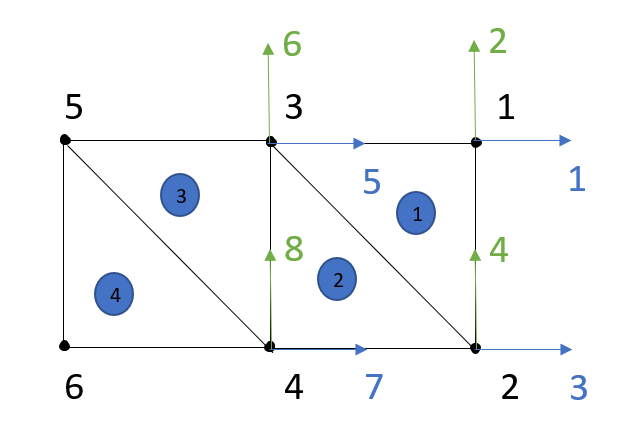
\includegraphics[width=0.6\textwidth,center]{fig/q2_prova2010.PNG}
	\caption{Numeração das equações.} 
	\label{provas:Numeracao_eq}
\end{figure}
%
\begin{itemize}
	\item b)	
\end{itemize}
%
A integral de forças no contorno é(pag. 22),
%
\begin{equation}
	\mathbf{f}_i = \int_{\Gamma} \mathbf{N}_i \mathbf{\bar t} d\Gamma
\end{equation}
%
em notação matricial temos,
%
\begin{equation}
	\begin{bmatrix}
		f^x_i\\
		f^y_i\\
	\end{bmatrix}
	=
	\int_{\Gamma}
	\begin{bmatrix}
		N_i&0\\
		0&N_i\\
	\end{bmatrix}
	\begin{bmatrix}
		q_x\\
		q_y\\
	\end{bmatrix}
	d\Gamma
	=
	\int_{\Gamma}
	\begin{bmatrix}
		N_i q_x\\
		N_i q_y\\
	\end{bmatrix}
	d\Gamma
	=
	\begin{bmatrix}
		\int_{\Gamma} N_i q_x d\Gamma\\
		\int_{\Gamma} N_i q_y d\Gamma
	\end{bmatrix}
\end{equation}
%
Como a força são uniformes nos bordos,
%
\begin{equation}
	\begin{bmatrix}
		f^x_i\\
		f^y_i\\
	\end{bmatrix}
	=
	\begin{bmatrix}
		\int_{\Gamma} N_i q_x d\Gamma\\
		\int_{\Gamma} N_i q_y d\Gamma
	\end{bmatrix}
\end{equation}
%
No problema $q_y = -q$ e $q_x = 0$, assim temos,
%
\begin{equation}
	\begin{bmatrix}
		f^x_i\\
		f^y_i\\
	\end{bmatrix}
	=
	\begin{bmatrix}
		0\\
		-q \int_{\Gamma} N_i d\Gamma
	\end{bmatrix}
\end{equation}
%
Funções de interpolação na aresta do triangulo,
%
\begin{equation}
	\begin{split}
		&N_1 = \xi_1 \\ 
		&N_2 = \xi_2 = (1 - \xi_1)
	\end{split}  
\end{equation}
%
As integrais são,
\begin{equation}
	\begin{split}
		&f_1^y = -q \int_{\Gamma} N_1 d\Gamma = -q \int_{0}^{1} N_1 det J d\xi_1 = -q L \int_{0}^{1} \xi_1 d\xi_1 = -\frac{q L}{2}\\
		&f_2^y = -q \int_{\Gamma} N_2 d\Gamma = -q \int_{0}^{1} N_2 det J d\xi_1 = -q L \int_{0}^{1} (1 - \xi_1) d\xi_1 =  -\frac{q L}{2}\\
	\end{split}
\end{equation}
%
Como $L = 1/2$, nos temos,
%
\begin{equation}
	\begin{split}
		&f_1^y = -\frac{q}{4}\\
		&f_2^y = -\frac{q}{4}\\
	\end{split}
\end{equation}
%
A equação 2 só tem a contribuição do elemento $1$ já a equações 6 tem a contribuição dos elementos $1$ e $3$. A força nodal equivalente é assim:

\color{blue}
Reposta:
\begin{equation}
	\mathbf{f} = \begin{bmatrix}0 & -\frac{q}{4} & 0 & 0 & 0 & -\frac{q}{2} & 0 & 0 \end{bmatrix}	
\end{equation}
\color{black}
%
\begin{itemize}
	\item c)	
\end{itemize}
%
\begin{figure}[H]
	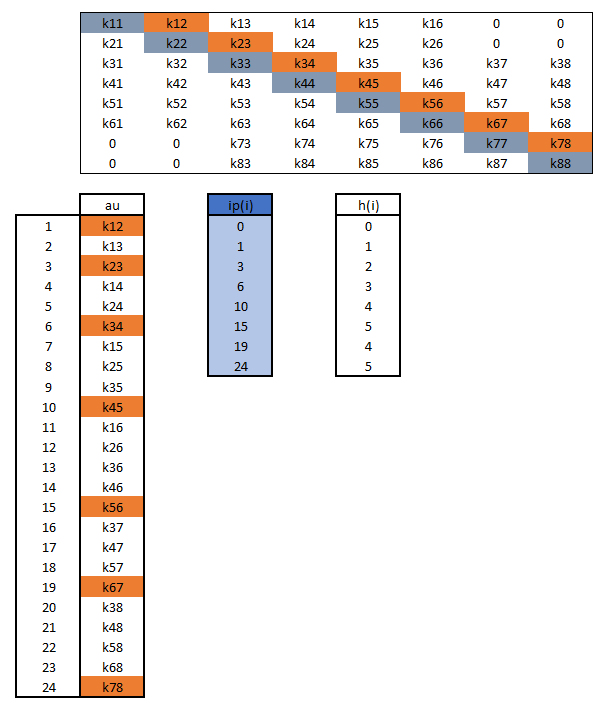
\includegraphics[width=1.0\textwidth,center]{fig/q2_prova2010_c.PNG}
	\caption{Perfil da matriz.} 
\end{figure}

\subsection{Q3 - prova - 2010}

A matriz $\mathbf{B}$ é dada por,

\begin{equation}
	\mathbf{B} =
	\begin{bmatrix}
	\mathbf{B}_1&  \mathbf{B}_2& \mathbf{B}_3
	\end{bmatrix}
\end{equation} 

onde as matrizes $\mathbf{B}_1$, $\mathbf{B}_2$ e $\mathbf{B}_3$ são dadas por,
%
\begin{equation}
	\mathbf{B_1} = \pounds \mathbf{N}_1 = 
	\begin{bmatrix}
		\mdp{N_1}{x}& 0\\
    	           0& \mdp{N_1}{y}\\
		\mdp{N_1}{y}& \mdp{N_1}{x}
	\end{bmatrix}
\end{equation}
%
\begin{equation}
	\mathbf{B_2} = \pounds \mathbf{N}_2 = 
	\begin{bmatrix}
		\mdp{N_2}{x}& 0\\
		0& \mdp{N_2}{y}\\
		\mdp{N_2}{y}& \mdp{N_2}{x}
	\end{bmatrix}
\end{equation}
%
\begin{equation}
	\mathbf{B_3} = \pounds \mathbf{N}_3 = 
	\begin{bmatrix}
		\mdp{N_3}{x}& 0\\
		0& \mdp{N_3}{y}\\
		\mdp{N_3}{y}& \mdp{N_3}{x}
	\end{bmatrix}
\end{equation}
%
Agora temos que calcular as derivadas das funções de interpolação. A relação entre as derivas em relação a $x$ e $y$ com as coordenadas locais $\xi_1$ e $\xi_2$ é dada pela inversa da matriz Jacobiana.
%
\begin{equation}
	\begin{bmatrix}
		\mdp{}{x}\\
		\mdp{}{y}
	\end{bmatrix} = J^{-1} 
	\begin{bmatrix}
	\mdp{}{\xi_1}\\
	\mdp{}{\xi_2}	
	\end{bmatrix}
	\label{provas:derivada_jacobiano}
\end{equation}
%
Para calcular a matriz inversa precisamos calcular A matriz Jacobina, para um de um triangulo linear temos,
%
\begin{equation}
J =	\begin{bmatrix}
		\mdp{x}{\xi_1}&\mdp{y}{\xi_1}\\
		\mdp{x}{\xi_2}&\mdp{y}{\xi_2}
	\end{bmatrix} =
    \begin{bmatrix}
  		x_1 - x_3&y_1 - y_3\\
	  	x_2 - x_3&y_2 - y_3
    \end{bmatrix} 
\end{equation}
%
Considerando a figura temos,
\begin{equation}
\begin{split}
x_1 = 1\\
y_1 = 0\\
x_2 = 0\\
y_2 = 1\\
x_3 = 0\\
y_3 = 0
\end{split}
\end{equation} 
% 
Portanto a matriz Jacobiana é dada por,
%
\begin{equation}
	J =	\begin{bmatrix}
		1&0\\
		0&1
		\end{bmatrix}
\end{equation}
%
A matriz inversa de uma matriz identidade é a própria matriz, ou seja,
%
\begin{equation}
	J^{-1} = J =	\begin{bmatrix}
		1&0\\
		0&1
	\end{bmatrix}
\end{equation}
%
Considerando agora a eq. (\ref{provas:derivada_jacobiano}) temos a relação entre as derivas da função $N_1$,
%
\begin{equation}
	\begin{bmatrix}
	\mdp{N_1}{x}\\
	\mdp{N_1}{y}
	\end{bmatrix}
     = 
	\begin{bmatrix}
	1&0\\
	0&1
	\end{bmatrix}          
	\begin{bmatrix}
	\mdp{N_1}{\xi_1}\\
	\mdp{N_1}{\xi_2}
	\end{bmatrix} 
\end{equation}
%
Sendo assim temos,
%
\begin{equation}
	\begin{split}
		\mdp{N_1}{x} = \mdp{N_1}{\xi_1}\\
		\mdp{N_1}{y} = \mdp{N_1}{\xi_2}
	\end{split}
\end{equation}
%
O mesmo raciocínio pode ser aplicado as funções $N_2$ e $N_3$, o que leva à,
%
\begin{equation}
	\begin{split}
		\mdp{N_2}{x} = \mdp{N_2}{\xi_1}\\
		\mdp{N_2}{y} = \mdp{N_2}{\xi_2}\\
		\mdp{N_3}{x} = \mdp{N_3}{\xi_1}\\
		\mdp{N_3}{y} = \mdp{N_3}{\xi_2}
	\end{split}
\end{equation}
%
Para o triangulo linear temos as seguintes funções de interpolação
%
\begin{equation}
	\begin{split}
		&N_1 = \xi_1\\ 
		&N_2 = \xi_2\\ 
		&N_3 = 1 - \xi_1 - \xi_2\\ 
	\end{split}
\end{equation}
%
Assim as derivas são,
%
\begin{equation}
	\begin{split}
		\mdp{N_1}{x} = 1\\
		\mdp{N_1}{y} = 0\\
		\mdp{N_2}{x} = 0\\
		\mdp{N_2}{y} = 1\\
		\mdp{N_3}{x} = -1\\
		\mdp{N_3}{y} = -1
	\end{split}
\end{equation}
%
A matriz $\mathbf{B}_1$, $\mathbf{B}_2$ e $\mathbf{B}_3$ ficam definidas como,
%
\begin{equation}
	\mathbf{B_1} = \pounds \mathbf{N}_1 = 
	\begin{bmatrix}
		1& 0\\
		0& 0\\
		0& 1
	\end{bmatrix}
\end{equation}
%
\begin{equation}
	\mathbf{B_2} = \pounds \mathbf{N}_2 = 
	\begin{bmatrix}
		0& 0\\
		0& 1\\
		1& 0
	\end{bmatrix}
\end{equation}
%
\begin{equation}
	\mathbf{B_3} = \pounds \mathbf{N}_3 = 
	\begin{bmatrix}
		-1& 0\\
		0& -1\\
		-1& -1
	\end{bmatrix}
\end{equation}
%
Portanto a $\mathbf{B}$ é,
%
\begin{equation}
	\mathbf{B} = 
	\begin{bmatrix}
		 1& 0   & 0 & 0 & -1 & 0\\
		 0& 0  & 0 & 1 &  0 & -1\\
		 0& 1  & 1 & 0 & -1 & -1
	\end{bmatrix}
\end{equation}
% 
O Calculo da deformação é dado por,
%
\begin{equation}
	\mathbf{\epsilon}(x, y) = 
	\begin{bmatrix}
	\varepsilon_x\\
	\varepsilon_y\\
	\gamma_{xy}	
	\end{bmatrix}
	 = 
	\begin{bmatrix}
		1& 0   & 0 & 0 & -1 & 0\\
		0& 0  & 0 & 1 &  0 & -1\\
		0& 1  & 1 & 0 & -1 & -1
	\end{bmatrix}
	\begin{bmatrix}
	u_1\\
	v_1\\
	u_2\\
	v_2\\
	u_3\\
	v_3\\	
    \end{bmatrix}
\end{equation}
%
Portanto,
\begin{equation}
	\mathbf{\epsilon}(x, y) = 
	\begin{bmatrix}
	\varepsilon_x\\
	\varepsilon_y\\
	\gamma_{xy}	
	\end{bmatrix}
	= 
	\begin{bmatrix}
	u_1 - u_3\\
	v_2 - v_3\\
	v_1 + u_2 - u_3 - v_3
	\end{bmatrix}
\end{equation}

\color{blue}
Reposta:
\begin{equation}
	\mathbf{B} = 
	\begin{bmatrix}
		1& 0   & 0 & 0 & -1 & 0\\
		0& 0  & 0 & 1 &  0 & -1\\
		0& 1  & 1 & 0 & -1 & -1
	\end{bmatrix}
\end{equation}
\begin{equation}
	\mathbf{\epsilon}(x, y) = 
	\begin{bmatrix}
		\varepsilon_x\\
		\varepsilon_y\\
		\gamma_{xy}	
	\end{bmatrix}
	= 
	\begin{bmatrix}
		u_1 - u_3\\
		v_2 - v_3\\
		v_1 + u_2 - u_3 - v_3
	\end{bmatrix}
\end{equation}
\color{black}


\textbf{Solução alternativa:}

As funções de interpolação do triangulo linear são sempre planos. Usando a figura podemos ver que os planos são fáceis de se obter, eles são:
%
\begin{equation}
	\begin{split}
		&N_1 = x\\ 
		&N_2 = y\\ 
		&N_3 = 1 - x - y\\ 
	\end{split}
\end{equation}
%
Assim as derivas são,
%
\begin{equation}
	\begin{split}
		\mdp{N_1}{x} = 1\\
		\mdp{N_1}{y} = 0\\
		\mdp{N_2}{x} = 0\\
		\mdp{N_2}{y} = 1\\
		\mdp{N_3}{x} = -1\\
		\mdp{N_3}{y} = -1
	\end{split}
\end{equation}
%
Agora todo o procedimento é igual ao anterior.

\color{red}

\textbf{Como chegar na relação $\mathbf{B}\mathbf{u}$}   

%
\begin{equation}
	\begin{bmatrix}
		\varepsilon_x\\
		\varepsilon_y\\
		\gamma_{xy} 	
	\end{bmatrix} = 
	\begin{bmatrix}
		\mdp{u}{x}\\
		\mdp{v}{y}\\
		\mdp{u}{y} + \mdp{v}{x} 	
	\end{bmatrix}
\end{equation}
%
\begin{equation}
	\begin{bmatrix}
		\varepsilon_x\\
		\varepsilon_y\\
		\gamma_{xy} 	
	\end{bmatrix} = 
	\begin{bmatrix}
		\mdp{N_1}{x} u_1+ \mdp{N_2}{x}  u_2+ \mdp{N_3}{x}  u_3\\
		\mdp{N_1}{y} v_1+ \mdp{N_2}{y}  v_2+ \mdp{N_3}{y}  v_3\\
		\mdp{N_1}{y} u_1+ \mdp{N_2}{y}  u_2+ \mdp{N_3}{y}  u_3 + \mdp{N_1}{x} v_1+ \mdp{N_2}{x} v_2 + \mdp{N_3}{x} v_3 	
	\end{bmatrix}
\end{equation}
%
\begin{equation}
	\begin{bmatrix}
		\varepsilon_x\\
		\varepsilon_y\\
		\gamma_{xy} 	
	\end{bmatrix} = 
	\begin{bmatrix}
		\mdp{N_1}{x}& 0           & \mdp{N_2}{x} & 0           & \mdp{N_3}{x}&           0 \\
		0           & \mdp{N_1}{y}&            0 & \mdp{N_2}{y}&            0& \mdp{N_3}{y} \\
		\mdp{N_1}{y}& \mdp{N_1}{x}& \mdp{N_2}{y} & \mdp{N_2}{x}& \mdp{N_3}{y}& \mdp{N_3}{x} 
	\end{bmatrix}
	\begin{bmatrix}
	u_1	\\
	v_1	\\
	u_2	\\
	v_2	\\
	u_3	\\
	v_3	\\
	\end{bmatrix}
\end{equation}
%
\begin{equation}
	\begin{bmatrix}
		\varepsilon_x\\
		\varepsilon_y\\
		\gamma_{xy} 	
	\end{bmatrix} = 
	\begin{bmatrix}
		\mathbf{B}_1& \mathbf{B}_2 & \mathbf{B}_3 
	\end{bmatrix}
	\begin{bmatrix}
		u_1	\\
		v_1	\\
		u_2	\\
		v_2	\\
		u_3	\\
		v_3	\\
	\end{bmatrix}
\end{equation}
%
\color{black}
%




\subsection{Q1 - prova - 2012}

A integral de forças no contorno é(pag. 22),
%
\begin{equation}
	\mathbf{f}_i = \int_{\Gamma} \mathbf{N}_i \mathbf{\bar t} d\Gamma
\end{equation}
%
em notação matricial temos,
%
\begin{equation}
	\begin{bmatrix}
		f^x_i\\
		f^y_i\\
	\end{bmatrix}
	=
	\int_{\Gamma}
	\begin{bmatrix}
		N_i&0\\
		0&N_i\\
	\end{bmatrix}
	\begin{bmatrix}
		q_x\\
		q_y\\
	\end{bmatrix}
	d\Gamma
	=
	\int_{\Gamma}
	\begin{bmatrix}
		N_i q_x\\
		N_i q_y\\
	\end{bmatrix}
	d\Gamma
	=
	\begin{bmatrix}
		\int_{\Gamma} N_i q_x d\Gamma\\
		\int_{\Gamma} N_i q_y d\Gamma
	\end{bmatrix}
\end{equation}
%
No problema $q_y = 0$ e $q_x$ é uma função linear, assim temos,
%
\begin{equation}
	\begin{bmatrix}
		f^x_i\\
		f^y_i\\
	\end{bmatrix}
	=
	\begin{bmatrix}
		\int_{\Gamma} N_i q_x d\Gamma\\
		0
	\end{bmatrix}
\end{equation}
%
\begin{itemize}
	\item Usando as funções de interpolação da barra
\end{itemize}
%
A função na aresta do elemento podem ser baseadas na Fig. \ref{provas:Lado do triangulo}. Funções quadraticas para $N$ e linear para $q_x$.
%
\begin{figure}[H]
	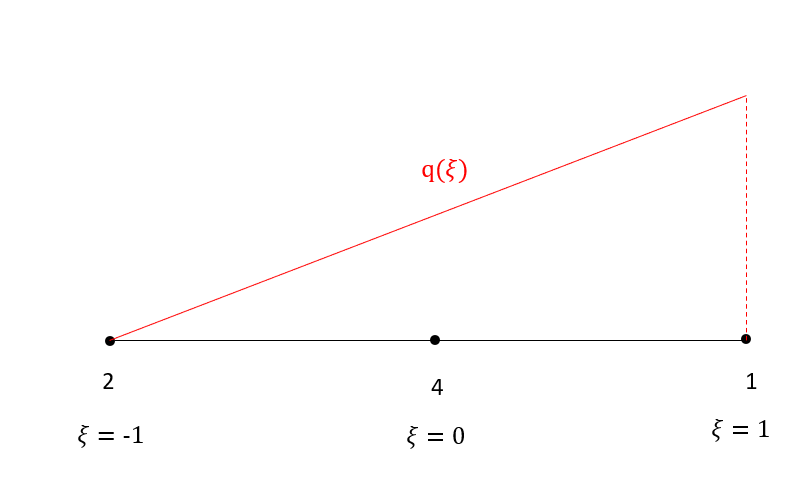
\includegraphics[width=0.6\textwidth,center]{fig/q1_prova_2012.PNG}
	\caption{Sistema de coordenadas da barra} 
	\label{provas:Lado do triangulo}
\end{figure}
%
Sendo assim,
%
\begin{equation}
	\begin{split}
	&N_2 = \frac{1}{2} \xi (\xi - 1) \\ 
	&N_4 = (1 + \xi) (1 - \xi) \\ 
	&N_1 = \frac{1}{2} \xi (1 + \xi)\\
	&q_x = \frac{q}{2} (1 + \xi)
	\end{split}  
\end{equation}
%
As integrais são,
\begin{equation}
	\begin{split}
		&f_2^x = \int_{\Gamma} N_2 q_x d\Gamma = \int_{-1}^{1} N_2 q_x det J d\xi = \frac{q L}{8} \int_{-1}^{1} \xi (\xi - 1) (1 + \xi) d\xi = 0\\
		&f_4^x = \int_{\Gamma} N_4 q_x d\Gamma = \int_{-1}^{1} N_4 q_x det J d\xi = \frac{q L}{4} \int_{-1}^{1} (1 + \xi)^2 (1 - \xi) d\xi =  \frac{q L}{3}\\
		&f_1^x = \int_{\Gamma} N_1 q_x d\Gamma = \int_{-1}^{1} N_1 q_x det J d\xi = \frac{q L}{8} \int_{-1}^{1} \xi (1 + \xi) (1 + \xi)  d\xi =  \frac{q L}{6}
	\end{split}
\end{equation}
%
 \begin{itemize}
	\item Usando as funções de interpolação do triangulo
\end{itemize}
%
Na Figura \ref{provas:coordenadas_de_area} temos as áreas utilizadas no sistema de coordenadas locais do triangulo. 
\begin{figure}[H]
	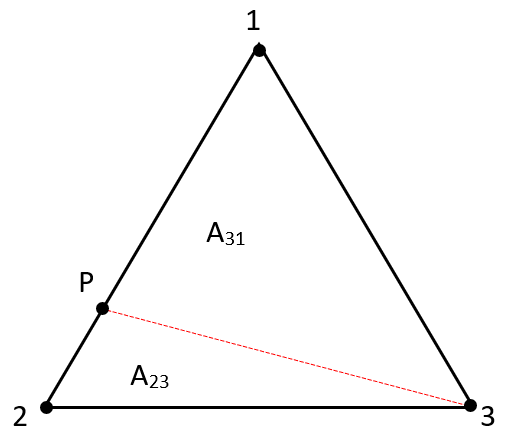
\includegraphics[width=0.6\textwidth,center]{fig/q1_triangulo_2012.PNG}
	\caption{Coordenadas de área do triângulo.} 
	\label{provas:coordenadas_de_area}
\end{figure}
%
Se o ponto $P$ só pode estar na aresta 1-2. Nos temos que
%
\begin{equation}
	\begin{split}
		&\xi_1 = \frac{A_{31}}{A} = \frac{A_{31}}{A}\\
    	&\xi_2 = \frac{A_{23}}{A} = \frac{A - A_{31}}{A} = 1 -  \frac{A_{31}}{A} = 1 - \xi_1\\
		&\xi_3 = \frac{A_{12}}{A} = 0
	\end{split}
\end{equation} 
%
A funções de interpolação são
%
\begin{equation}
	\begin{split}
		&N_1 = \xi_1 (2 \xi_1 - 1) \\ 
		&N_4 = 4 \xi_1 \xi_2 = 4 \xi_1 (1 - \xi_1)\\ 
		&N_2 = \xi_2 (2 \xi_2 - 1) = (1 - \xi_1) (1 - 2 \xi_1)\\
		&q_x = q \xi_1
	\end{split}  
\end{equation}
%
As integrais são,
\begin{equation}
	\begin{split}
		&f_2^x = \int_{\Gamma} N_2 q_x d\Gamma = \int_{0}^{1} N_2 q_x det J d\xi = q L \int_{0}^{1} (1 - \xi_1) (1 - 2 \xi_1) \xi_1 d\xi = 0\\
		&f_4^x = \int_{\Gamma} N_4 q_x d\Gamma = \int_{0}^{1} N_4 q_x det J d\xi = 4 q L \int_{0}^{1} \xi_1 (1 - \xi_1) \xi_1 d\xi =  \frac{q L}{3}\\
		&f_1^x = \int_{\Gamma} N_1 q_x d\Gamma = \int_{0}^{1} N_1 q_x det J d\xi = q L \int_{0}^{1} \xi_1 (2\xi_1 - 1) \xi_1  d\xi =  \frac{q L}{6}
	\end{split}
\end{equation}
%
\color{blue}
Reposta:
\begin{equation}
	\begin{split}
		&\mathbf{f}_2
		= 
		\begin{bmatrix}
			0\\
			0
		\end{bmatrix}\\
		&\mathbf{f}_4
		= 
		\begin{bmatrix}
			\frac{q L}{3}\\
			0
		\end{bmatrix}\\
		&\mathbf{f}_1
		= 
		\begin{bmatrix}
		\frac{q L}{6}\\
		0
	\end{bmatrix}\\	
	\end{split}
\end{equation} 
\color{black}
%
A força resultante da aresta é $\frac{q L}{2}$. Para verificar a resposta vamos somar $f_1^x$, $f_2^x$ e $f_4^x$ para calcular a força resultante na aresta através das forças equivalentes nodai,
%
\begin{equation}
	f_r^x = f_1^x + f_2^x + f_4^x = \frac{q L}{6} + \frac{q L}{3} + 0 = \frac{q L}{2}
\end{equation}


\subsection{Q2 - prova - 2012}

Utilizando o meto do resíduos ponderados temos,
%
\begin{equation}
	\int_{\Omega} \left[k \left(\mdpv{\phi}{x} + \mdpv{\phi}{y}\right) + Q\right]w d\Omega = 0	
\end{equation}
%
Expandindo as integral temos,
%
\begin{equation}
	\int_{\Omega} k \mdpv{\phi}{x} w d\Omega + \int_{\Omega} k \mdpv{\phi}{y} w d\Omega + \int_{\Omega} Q w d\Omega = 0
	\label{provas:passo_intermediario}
\end{equation}
%
O objetivo agora é diminuir a ordem da deriva de $\phi$, nós queremos apenas derivadas primeira em $\phi$. Pelo teorema do divergente temos,
%
\begin{equation}
	\begin{split}
	&\int_{\Omega} \mdp{} {x} \left( k \mdp{\phi}{x} w \right) d\Omega = \int_{\Gamma} \left(k \mdp{\phi}{x}\right) w n_x d\Gamma\\
	&\int_{\Omega} \mdp{} {y} \left( k \mdp{\phi}{y} w \right) d\Omega = \int_{\Gamma} \left(k \mdp{\phi}{y}\right) w n_y d\Gamma
    \end{split}
	\label{provas:gauss}
\end{equation}
%
Pela integra por partes temos,
%
\begin{equation}
	\begin{split}
	&\int_{\Omega} \mdp{} {x} \left( k \mdp{\phi}{x} w \right) d\Omega = \int_{\Omega} k \mdpv{\phi}{x} w d\Omega + \int_{\Omega} k \mdp{\phi}{x} \mdp{w} {x}  d\Omega\\
	&\int_{\Omega} \mdp{} {y} \left( k \mdp{\phi}{y} w \right) d\Omega = \int_{\Omega} k \mdpv{\phi}{y} w d\Omega + \int_{\Omega} k \mdp{\phi}{y} \mdp{w} {y}  d\Omega\\
	\end{split}
	\label{provas:partes}
\end{equation}
%
Juntando a eq. (\ref{provas:gauss}) e eq. (\ref{provas:partes}),
%
\begin{equation}
	\begin{split}
		&\int_{\Gamma} \left(k \mdp{\phi}{x}\right) w n_x d\Gamma = \int_{\Omega} k \mdpv{\phi}{x} w d\Omega + \int_{\Omega} k \mdp{\phi}{x} \mdp{w} {x}  d\Omega\\
		&\int_{\Gamma} \left(k \mdp{\phi}{y}\right) w n_y d\Gamma = \int_{\Omega} k \mdpv{\phi}{y} w d\Omega + \int_{\Omega} k \mdp{\phi}{y} \mdp{w} {y}  d\Omega\\
	\end{split}
\end{equation}
%
Rearranjando os termos,
%
\begin{equation}
	\begin{split}
		&\int_{\Omega} k \mdpv{\phi}{x} w d\Omega = \int_{\Gamma} \left(k \mdp{\phi}{x}\right) w n_x d\Gamma - \int_{\Omega} k \mdp{\phi}{x} \mdp{w} {x} d\Omega\\
		&\int_{\Omega} k \mdpv{\phi}{y} w d\Omega = \int_{\Gamma} \left(k \mdp{\phi}{y}\right) w n_y d\Gamma - \int_{\Omega} k \mdp{\phi}{y} \mdp{w} {y} d\Omega\\
	\end{split}
	\label{provas:divergente+partes}
\end{equation}
%
Agora com a eq. (\ref{provas:divergente+partes}) podemos voltar para a eq. (\ref{provas:passo_intermediario})
%
\begin{equation}
	\begin{aligned}
	&\int_{\Gamma} \left(k \mdp{\phi}{x}\right) w n_x d\Gamma + \int_{\Gamma} \left(k \mdp{\phi}{y}\right) w n_y d\Gamma - \int_{\Omega} k \mdp{\phi}{y}\mdp{w}{y} d\Omega\\
	& - \int_{\Omega} k \mdp{\phi}{x} \mdp{w}{x} d\Omega + \int_{\Omega} Q w d\Omega = 0 
	\end{aligned}
\end{equation}
%
Rearranjando os termos,
%
\begin{equation}
\int_{\Omega} k \left(\mdp{\phi}{x} \mdp{w}{x} + \mdp{\phi}{y} \mdp{w}{y} \right) d\Omega = \int_{\Gamma} k \left(\mdp{\phi}{x} n_x + \mdp{\phi}{y} n_y \right) w d\Gamma + \int_{\Omega} Q w d\Omega 
\end{equation}
%
Considerando agora a condição de contorno natural,
%
\begin{equation}
	q = k \mdp{\phi}{n} = k \left(\mdp{\phi}{x} n_x + \mdp{\phi}{y} n_y\right)
\end{equation}
%
A formulação variacional final é (pag. 168),

\color{blue}
Reposta a):
\begin{equation}
	\int_{\Omega} k \left(\mdp{\phi}{x} \mdp{w}{x} + \mdp{\phi}{y} \mdp{w}{y} \right) d\Omega = \int_{\Gamma_2} q w d\Gamma + \int_{\Omega} Q w d\Omega 
\end{equation}
\color{black}
%
%
\begin{itemize}
	\item Questão b)
\end{itemize}
%
Definindo as aproximações para $\phi$ e $w$,
% 
\begin{equation}
	\begin{split}
		&\phi = \sum_{j=0}^n N_j \phi_j\\
		&w = \sum_{i=0}^n N_i w_i
	\end{split}
\end{equation}
%
Substituindo na resposta a) chega-se à:

\color{blue}
Reposta b):
\begin{equation}
	\begin{split}
		&k_{ij} = \int_{\Omega} k \left( \mdp{N_j}{x}\mdp{N_i}{x} + \mdp{N_j}{y}\mdp{N_i}{y} \right) d \Omega\\
		&f_{i} = \int_{\Gamma_2} q N_i d\Gamma + \int_{\Omega} Q N_i d \Omega
	\end{split}
\end{equation}
\color{black}
%
\begin{itemize}
	\item Questão c)
\end{itemize}

Como as derivada que aparecem na integral de omega são de primeira ordem temos que as funções aproximação precisam ser da classe $C^0$ pela condição de compatibilidade. Isso implica que as aproximação que ser no mínimo linear. A outra condição é de completidade, as aproximações tem que ser um polinômio completo. Ou seja tem que ser da forma:

\begin{equation}
A_p x^p + A_{p-1} x^{p-1} + A_{p-2}x^{p-2} ... + A_1 x + A_0 x^0
\end{equation}



\subsection{Q3 - prova - 2012}

A área do retângulo pode ser escrita na forma de uma integral. Além disso o determinante da jacobiano de uma paralelogramo é constante, assim temos,
%
\begin{equation}
	\begin{split}
		&A = \int_A dA = \int_{-1}^{1} \int_{-1}^{1} det J d\eta d\xi\\
		&A = det J \int_{-1}^{1} \int_{-1}^{1} d\eta d\xi\\
		&A = det J 4
	\end{split}
\end{equation}
%
\color{blue}
Reposta:
\begin{equation}
	det J = \frac{A}{4}
\end{equation} 
\color{black}
